\clearpage
\section{Auswertung}

\subsection{Messung der Homogenität des Magnetfeldes mit der Hallsonde}

Wir haben die Homogenität des Permanentmagneten untersucht, indem wir eine Hallsonde zwischen den Stirnflächen positioniert und dann einmal horizontal und einmal vertikal mit dieser entlang der Stirnflächen gefahren sind und die Stärke des Magnetfeldes mit einem Teslameter an jeder Stelle gemessen haben.

Für den horizontalen Teil haben wir die Mitte der Stirnflächen in y-Richtung als $y_c = 15.45\ cm$ abgeschätzt. Beim vertikalen Teil haben wir dann $x_c = 8.00\ cm$ benutzt.

Eine erste horizontale Messung erfolgte sehr schnell, jedoch haben wir dann gemerkt, dass das Teslameter einige Zeit benötigte um sich auf einen festen Wert einzustellen und mussten also die Messung noch einmal wiederholen, diesmal mit längerer Zeit pro Messpunkt. Auch bei dieser zweiten Messung hatte das Teslameter einige Probleme, nämlich stieg die Anzeige manchmal zuerst auf sehr hohe Werte (etwa 460 - 490 mT), bevor sie sich wieder auf reelle Werte festgelegt hat. (Dies dauerte z.T. einige Minuten). Unsere Ergebnisse sind wie folgt:

\begin{figure}[H]
\centering 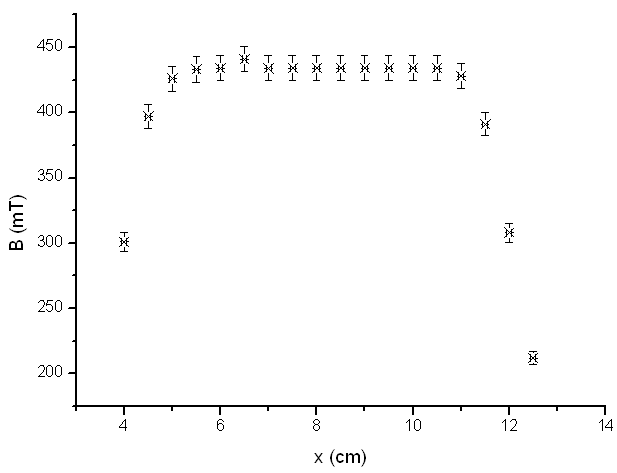
\includegraphics[width=\textwidth]{Bilder/Hallx.png}
\caption{Horizontale Messung}
\end{figure}

\begin{figure}[H]
\centering 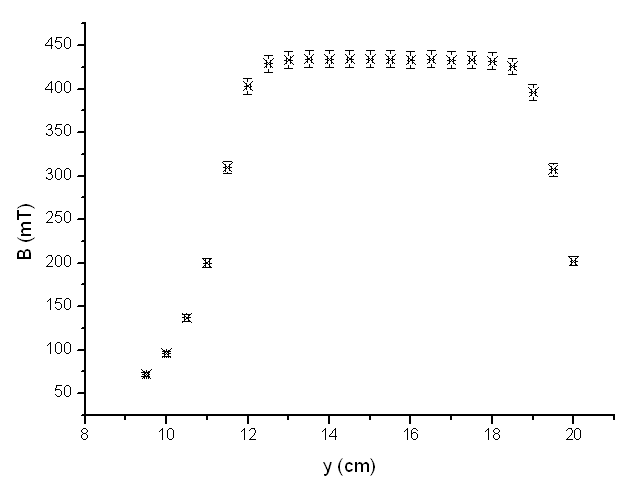
\includegraphics[width=\textwidth]{Bilder/Hally.png}
\caption{Vertikale Messung}
\end{figure}

Den Fehler auf x oder y haben wir mit $s_x=s_y=0.05\ cm$ geschätzt. Der Fehler auf das Teslameter wurde uns mit 2\% und 1 Digit angegeben. Durch (gewichtete) Mittelwertbildung der Plateaus haben wir somit die Magnetfeldstärke im homogenen Bereich ermitteln können, nämlich gilt:

$$\boxed{B = (434.1 \pm 4.5) mT}$$

\subsection{Messung der Resonanzfrequenzen der 3 Proben}

Das sinusförmig modulierte Magnetfeld des Permanentmagneten haben wir als Trigger auf dem Oszilloskop benutzt, um das Absorptionssignal zu stabilisieren. Dann haben wir die Frequenz so eingestellt, dass die Absorptionslinien äquidistant waren und diese gemessen. Für den Fehler haben wir uns überlegt, wie weit wir die Frequenz verändern konnten, bis dass das Muster nicht mehr äquidistant aussah. Bei der Wasserstoff- und der Teflonprobe war dies bereits nach 2 kHz Veränderung klar erkennbar, bei der Glykolprobe hatten wir jedoch schon Probleme die Absorptionslinien klar vom Rauschen trennen zu können und haben deswegen den Fehler ziemlich groß geschätzt. Unsere Resultate sind, mit angehängtem Absorptionsspektrum:

\bildfreq{glykol}{18.184}{0.050}
\bildfreq{H}{18.180}{0.002}
\bildfreq{teflon}{17.114}{0.002}

\subsection{Berechnung von gyromagnetischem Verhältnis und kernmagnetischem Moment}

Aus Gleichung (\ref{g}) folgt sofort, dass:

\begin{equation} g_K = \frac{h\cdot\nu_r}{\mu_K\cdot B} \end{equation}

mit dem Fehler $$s_{g_K} = g_K\sqrt{\frac{s_\nu^2}{\nu^2}+\frac{s_B^2}{B^2}}$$

Aus $g_K$ kann dann das gyromagnetische Verhältnis berechnet werden:

$$\gamma  \stackrel{(\ref{gyro})}{=} \frac{g_K\cdot\mu_K}{\hbar}$$

mit dem Fehler:

$$s_\gamma = \gamma \frac{s_{g_K}}{g_K}$$

Wir haben die Ergebnisse in einer Tabelle zusammengefasst:

\begin{center}
\begin{tabular}{| l | c | c | c | c |} \hline
Probe & $\nu_r$ / MHz & $g_K$ & $\sigma(g)$ & $\gamma\ / MHz\cdot T^{-1}$\\ \hline
Glykol & $18.184 \pm 0.050$ & $5.495 \pm 0.059$ & 2 & $263.2 \pm 2.8$ \\
Wasserstoff &$18.180 \pm 0.002$ & $ 5.494 \pm 0.057 $ & 2 & $263.2 \pm 2.7$ \\
Teflon & $17.114 \pm 0.002$ &  $5.172 \pm 0.054$ & 2 & $247.7 \pm 2.6$\\ \hline
\end{tabular}
\end{center}

$\sigma(g)$ beschreibt in der wievielten Standardabweichungen der theoretische Wert für $g$ liegt mit: $g_{lit,F} = 5.2577$ und $g_{lit,H} = 5.5856$

Für die Teflonprobe berechnen wir zusätzlich noch exemplarisch das kernmagnetische Moment $\mu_K$, indem wir den Wert für $g$ als gegeben annehmen. Somit folgt für das kernmagnetische Moment aus (\ref{g}):

$$\mu_K =  \frac{h\cdot\nu_r}{g_{lit}\cdot B} = 4.968\cdot 10^{-27} J/T$$

$$s_{\mu_K} = \mu_K\sqrt{\frac{s_\nu^2}{\nu^2} + \frac{s_B^2}{B^2}} = 0.052\cdot 10^{-27} J/T$$

Der Literaturwert beträgt $\mu_{lit} = 5.051 \cdot 10^{-27} J/T$ und liegt somit in der 2. Standardabweichung.

\subsection{Messung der Homogenität des Magnetfeldes mit der Wasserstoffprobe}

Da die Wasserstoffprobe sich als die Probe herausgestellt hat, bei der man das Absorptionsmuster am besten sehen konnte, haben wir sie benutzt um erneut die Homogenität des Magnetfeldes des Permanentmagneten zu messen. Wir haben den gleichen festen $y$-Wert wie bei der Hall-Sonde benutzt, also $y_{fest} = 15.45 cm$ bei der horizontalen Messung. Für den $x$-Wert bei der vertikalen Messung haben wir den Längenunterschied zwischen der Hallsonde und dem Probenstab gemessen ($\Delta x = 5.8 cm$) und diesen zu dem festen $x$-Wert von der ersten Messung addiert. Somit folgt $x_{fest} = 13.8 cm$ bei der vertikalen Messung.

Im Gegensatz zu der Messung mit der Hallsonde haben wir die Position der Probe verändert und die Frequenz nachgeführt, so dass wir wie bei 4.2. ein äquidistantes Absorptionsspektrum erhielten, also die Resonanzfrequenz getroffen haben. Aus dieser haben wir dann mit Gl. (\ref{g}) das Magnetfeld berechnen können. 

Da die Resonanz an den Randstellen des vorhin ermittelten Plateaus der Magnetfeldstärke nicht mehr zu finden war (das Verstellen der Frequenz war begrenzt), haben wir nur das Plateau gemessen. Hier die Ergebnisse:

\begin{figure}[H]
\centering 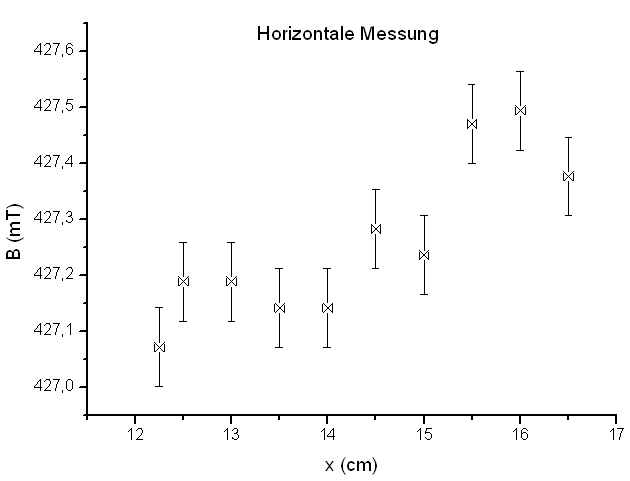
\includegraphics[width=0.8\textwidth]{Bilder/homhor.png}
\caption{Horizontale Messung}
\end{figure}

\begin{figure}[H]
\centering 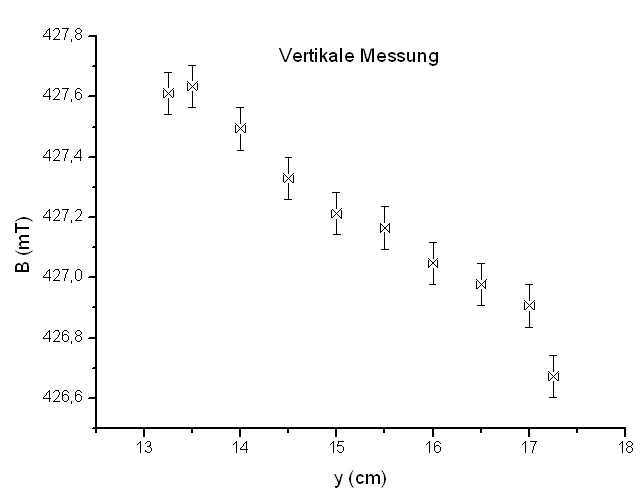
\includegraphics[width=0.8\textwidth]{Bilder/homvert.png}
\caption{Vertikale Messung}
\end{figure}

Man kann eine leichte Linearität erkennen. Die Fehler auf die Frequenz wurden mit $s_\nu=3\ kHz$ abgeschätzt, auf die Position mit $s_x=s_y=0.05cm$.

\subsubsection{Vergleich beider Magnetfeldmessungen}

\begin{figure}[H]
\centering 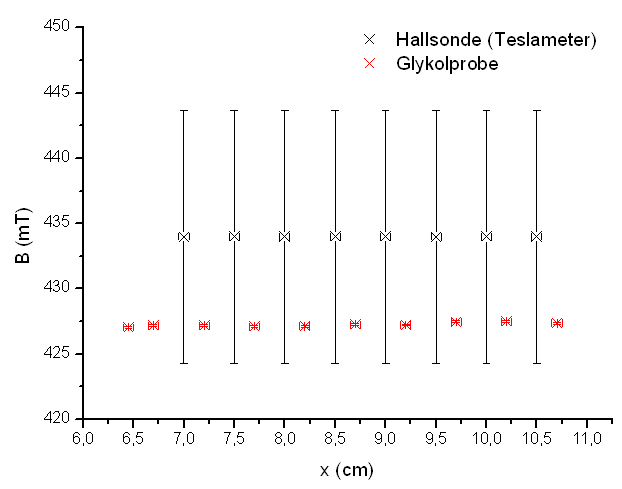
\includegraphics[width=0.65\textwidth]{Bilder/VGLx.png}
\caption{Horizontale Messung}
\end{figure}

\begin{figure}[H]
\centering 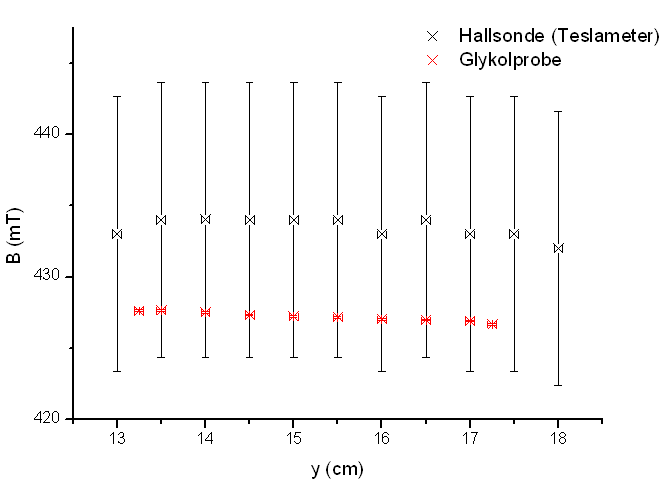
\includegraphics[width=0.65\textwidth]{Bilder/VGLy.png}
\caption{Vertikale Messung}
\end{figure}

Das mit der Glykolprobe gemessene Magnetfeld ist also systematisch kleiner als das mit der Hallsonde und dem Teslameter ermittelte. %..........blabla ;) Ich weiss nicht genau was!

\subsection{Resonanzfrequenzbestimmung mit der Lock-In-Methode}

Die Messung mit der Lock-In-Methode wurde bei $x=13.8cm$ und $y=15.45cm$ durchgeführt. Wir haben wiederum die Wasserstoffprobe benutzt. Das Magnetfeld wurde mit einem Sägezahn moduliert, der selber mit einem hochfrequenten Sinus moduliert wurde. Zur Messung der Resonanzfrequenz haben wir verschiedene Frequenzen eingestellt und dann die Distanz des Resonanzpunktes zum Sägezahnanfang gemessen. Die Sägezahnbreite betrug $b = (10.810 \pm 0.010)s$. 

Da wir den Nullpunkt des Sägezahns nicht kennen, haben wir aus den gemessenen Abständen zu dessen Anfang und der Länge des Sägezahns die Distanz des Signals zum Ende berechnen können. Wir haben beide Distanzen in ein Diagramm geplottet und linear gefittet. Der Schnittpunkt der Geraden ist genau der Nulldurchgang und dessen Ordinate entspricht dann der Resonanzfrequenz der Wasserstoffprobe.

Den Fehler auf den Abstand zum Anfang beträgt $s_{AA}=0.010$ und zum Ende $s_{AE}=0.014$, wegen dem Fehler auf die Sägezahnbreite. Den Fehler auf die Frequenz schätzen wir mit $s_\nu$ = 0.002 MHz.

\begin{figure}[H]
\centering 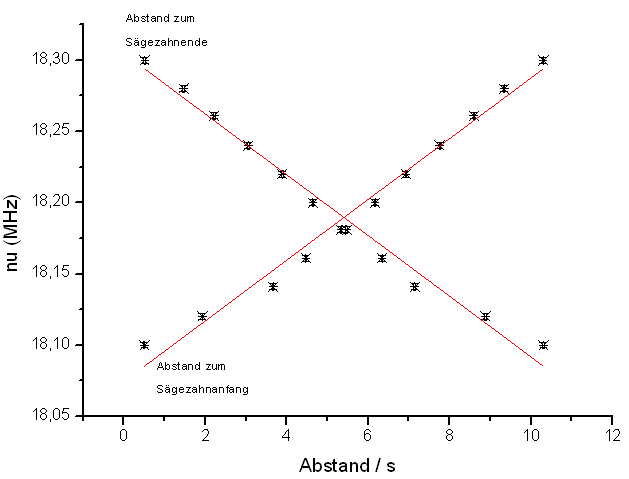
\includegraphics[width=0.99\textwidth]{Bilder/linreg.png}
\caption{Linearer Fit der Messung mit dem Lock-In-Verfahren}
\end{figure}

Wir erhalten folgende Geradengleichungen

$$ y_{AA} = (0.021 \pm 0.001)x + (18.074 \pm 0.006) $$
$$ y_{AE} = -(0.021 \pm 0.001)x + (18.305 \pm 0.005) $$

Der Schnittpunkt der Geraden, die Resonanzfrequenz, ist also einfach der Mittelwert zwischen den Achsenabschnitten:

$$ \boxed{\nu_r = \frac{18.074 + 18.305}{2} = 18.190 MHz} $$

Mit dem Fehler:

$$s_{\nu_r} = \frac{1}{2}\sqrt{0.006^2 + 0.005^2} = 0.004$$

Als Vergleich mit dem Wert aus der Messung in 4.2. haben wir eine Abweichung von 0.055\% und einen Unterschied von 3 Standardabweichungen.

Hieraus können wir auch wiederum den Wert für g berechnen und erhalten:

$$ g = \frac{h\cdot\nu_r}{\mu_K\cdot B} \pm g_K\sqrt{\frac{s_\nu^2}{\nu^2} + \frac{s_B^2}{B^2}} = 5.497 \pm 0.057 $$ 

welcher in der 2. Standardabweichung des Literaturwerts liegt.













